% control regions, transfer factors
% binning in razor variables
% statistical treatment and systematic uncertainties

\begin{figure}[htpb]
  \centering
  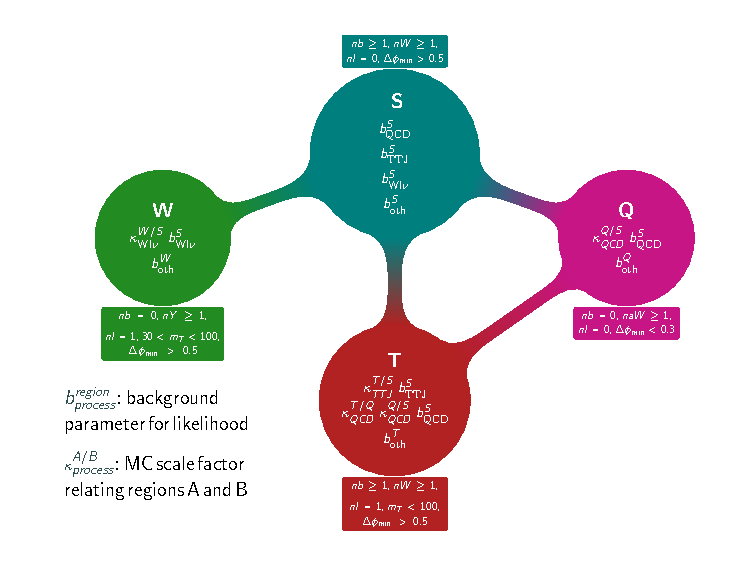
\includegraphics[width=\textwidth]{figures/razor_strategy/BoostFlowChart_noZ}
  \caption{
  \label{fig:boost_flowchart}}
\end{figure}


% In light of the discussion above, it is expected that boosted top quarks are a promising signature
% of new physics involving a massive gluino decaying to a relatively light top squark.  
% Boosted objects with high transverse momentum, $\pt$, are characterized by merged decay products
% separated by $ \delta R {\sim} 2 m / \pt $, where $m$ and $\pt$ denote the mass and transverse
% momentum of the mother particle. 
% For a separation of $\delta R = 0.5$, a top quark should have a momentum of ${\sim}700$\GeV,
% a value difficult to reach with proton-proton collisions at 8 TeV.  Therefore, in order to
%increase
% the signal efficiency, we consider instead $\PW$ bosons from top quark decays, which are required
%to
% have a more accessible $\pt {\sim} 320$\GeV.  The final state
% therefore contains boosted $\PW$ bosons and jets originating from $\cPqb$ quarks (\ie $\cPqb$
%jets).
%  Hadronically decaying boosted $\PW$ boson candidates are identified using pruned jet
% mass~\cite{Ellis:2009su,Ellis:2009me,Chatrchyan:2013vbb} and a jet substructure observable
% called N-subjettiness \cite{Thaler:2010tr}, while the razor kinematic variables \cite{rogan} are
% used to discriminate processes with new heavy  particles and missing energy from standard model
% processes. We perform the search in a binned region defined by the razor variables.  

% This paper is organized as follows.
% The razor variables are introduced in Section~\ref{sec:razor}. Section~\ref{sec:cms} gives a brief
% overview of the CMS detector, while Section~\ref{sec:triggerdatasets} covers the triggers,
%datasets,
% and Monte Carlo (MC) simulated samples used in this analysis.  
% Details of the object definitions and event selection are given in Sections~\ref{sec:eventreco}
%and
% \ref{sec:selection}, respectively.
% The statistical analysis is explained in Section~\ref{sec:likelihood} and
% Section~\ref{sec:systematics} covers the systematic uncertainties.  Finally, our results and their
% interpretation are presented in Section~\ref{sec:interpretation}. 

